% Author:Zhuming Shi, Peking University
% Theme from https://github.com/matze/mtheme

\documentclass[12pt,AutoFakeBold]{beamer}
\usepackage[english]{babel}

\usetheme{metropolis}

\usepackage{xeCJK} % Chinese support
\setCJKmainfont{SimSun} % Chinese front
\usepackage{booktabs}%绘制三线表

\usepackage{fontspec}%控制字体
\setmainfont{Times New Roman}%英文字体
\newfontfamily\arial{Arial}%Arial字体
\usepackage{xeCJK}%控制中文
\setCJKmainfont{SimSun}%中文字体
\XeTeXlinebreaklocale "zh"%中文自动换行
\XeTeXlinebreakskip = 0pt plus 1pt%中文自动换行

\usepackage{booktabs}%绘制三线表
\usepackage{latexsym}%绘制特殊数学符号
\usepackage{siunitx}%数学模式中使用SI单位

\usepackage{hyperref}%超链接

\usepackage{media9}

\title{重返事故现场}
\author{北大车协车队\ 施朱鸣}
\date{2020年4月14日}

% \usepackage[orientation=landscape,size=custom,width=16,height=9,scale=0.5,debug]{beamerposter}%修改比例,16:9

\usepackage{graphicx} 

\begin{document}
    {
    \usebackgroundtemplate{\includegraphics[width=\paperwidth,height=\paperheight]{figures/cover.jpg}}
    \begin{frame}
    \end{frame}
    }

    \frame[plain]{\titlepage}

    \frame{\frametitle{Outline}\tableofcontents[hideallsubsections]}
    % \begin{frame}
    %     \frametitle{别人的事故视频}
    %     \textbf{BGM嘈杂,请静音}
    %     \includemedia[width=0.8\linewidth,height=0.6\linewidth]{}{figures/after.mp4}
    % \end{frame}

    \section{我的经历}

    \begin{frame}
        \frametitle{事故之前}
    
        \begin{itemize}
            \item 刚刚考完一门期末考试
            \item 背了一下午明天的考试
            \item 不想背书了,想骑车去了
        \end{itemize}
    
    \end{frame}

    \begin{frame}
        \frametitle{地形和数据}
        \begin{center}
            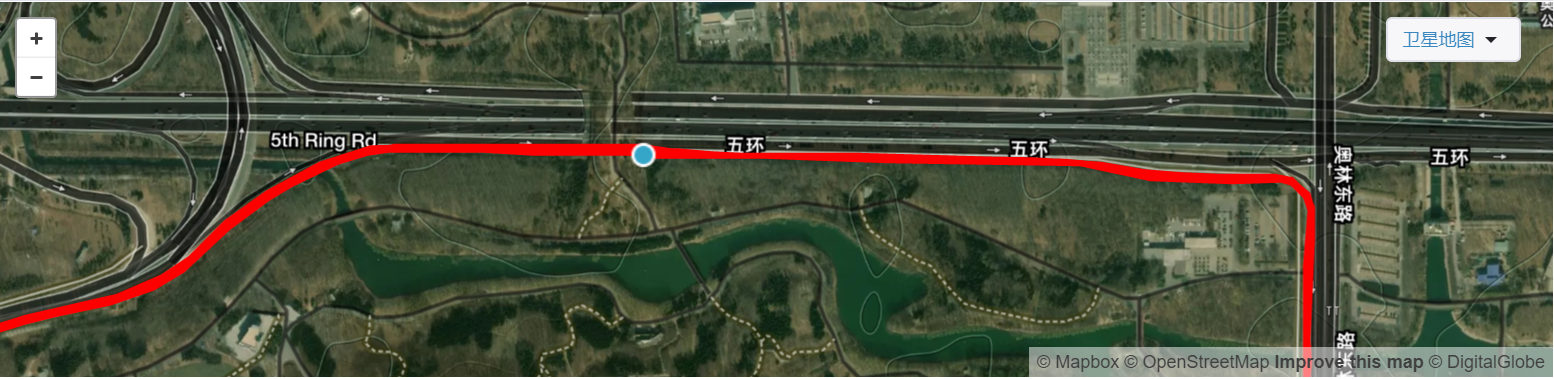
\includegraphics[width=0.8\paperwidth]{figures/map.png}
            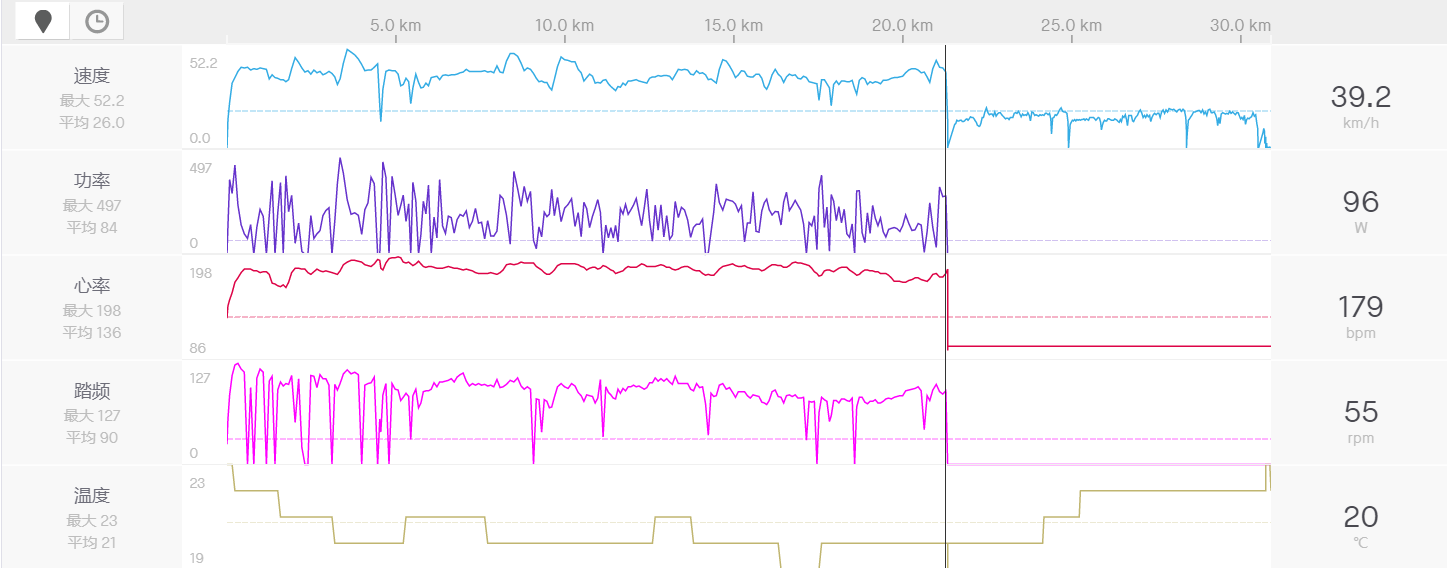
\includegraphics[width=0.8\paperwidth]{figures/table.png}
        \end{center}
    \end{frame}

    \begin{frame}
        \frametitle{事故处理}
        \begin{itemize}
            \item 6月5日22:00:120急救车运送,队友陪同
            \item 6月6日1:00:北医三院,车协主席陪同
            \item 6月10日18:00:接受手术治疗
            \item 6月14日8:30:考完有机期末回家休整
        \end{itemize}
        \begin{center}
            \textbf{感谢学院、协会和车队的帮助!}
        \end{center}
    \end{frame}

    \begin{frame}
        \frametitle{复习:骨折紧急处理}
        本部分内容选自北大车协《队医宝典初阶版\ 1.0版》
        
        专有表现:畸形、异常活动、骨擦音或骨擦感

        一般表现:运动功能丧失、剧烈疼痛、肿胀、皮肤变色、淤斑
    \end{frame}

    \begin{frame}
        \frametitle{复习:骨折紧急处理}
        固定:
        \begin{itemize}
            \item 用树枝、木板、塑料板、厚纸板等固定伤肢的上下关节
            \item 关节间、骨折处加软垫
            \item 骨断端已暴露在外的开放性骨折,不可将断端回纳入伤口,用干净的敷料包扎
        \end{itemize}
        
        搬运:
        \begin{itemize}
            \item 尽可能使用硬担架,动作平稳,避免造成二次伤害
            \item 脊髓损伤:
            \begin{itemize}
                \item 强烈怀疑:肢体无力、麻木,脊柱疼痛,头外伤,多系统损伤
                \item 处理:只制动,不移动(移动整个脊柱)
            \end{itemize}
        \end{itemize}
    \end{frame}

    \begin{frame}
        \frametitle{后续影响}
        \begin{itemize}
            \item 暑假休息3个月,训练成果基本归零
            \item 喜提(划去)缓考重修大礼包
        \end{itemize}
        \begin{center}
            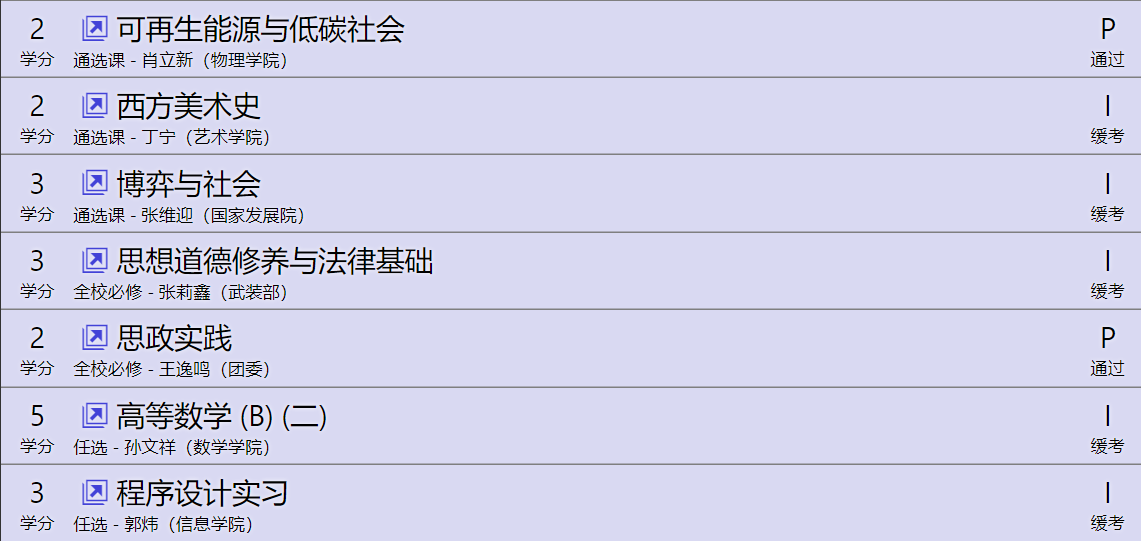
\includegraphics[width=0.618\paperwidth]{figures/result.png}    
        \end{center}
        
    \end{frame}

    \section{我的反思}
    \begin{frame}
        \frametitle{反思}
        \begin{itemize}
            \item \textbf{不要在状态不好的时候训练}
            \item \textbf{一定要戴头盔}
            \item \textbf{一定要购买保险}
            \item 在期末季等关键时间段避免中高风险运动
        \end{itemize}
    \end{frame}

    \section{结语}
    \begin{frame}
        \frametitle{结语}
        祝大家出行平安,享受骑行的乐趣。

        欢迎加入北大车协车队,北京大学场地车代表队!

        谢谢!

        本演示文稿开源于\href{https://github.com/ShiZhuming/CyclingEducation}{https://github.com/ShiZhuming/CyclingEducation}
    \end{frame}
\end{document}